\documentclass[paper=letter,11pt]{scrartcl}

\KOMAoptions{headinclude=true, footinclude=false}
\KOMAoptions{DIV=14, BCOR=5mm}
\KOMAoptions{numbers=noendperiod}
\KOMAoptions{parskip=half}
\addtokomafont{disposition}{\rmfamily}
\addtokomafont{part}{\LARGE}
\addtokomafont{descriptionlabel}{\rmfamily}
%\setkomafont{pageheadfoot}{\normalsize\sffamily}
\setkomafont{pagehead}{\normalsize\rmfamily}
%\setkomafont{publishers}{\normalsize\rmfamily}
\setkomafont{caption}{\normalfont\small}
\setcapindent{0pt}
\deffootnote[1em]{1em}{1em}{\textsuperscript{\thefootnotemark}\ }


\usepackage{amsmath}
\usepackage[varg]{txfonts}
\usepackage[T1]{fontenc}
\usepackage{graphicx}
\usepackage{xcolor}
\usepackage[american]{babel}
% hyperref is needed in many places, so include it here
\usepackage{hyperref}

\usepackage{xspace}
\usepackage{multirow}
\usepackage{float}


\usepackage{braket}
\usepackage{bbm}
\usepackage{relsize}
\usepackage{tcolorbox}

\def\ketY{\ensuremath{\ket {\Psi}}}
\def\iGeV{\ensuremath{\textrm{GeV}^{-1}}}
%\def\mp{\ensuremath{m_{\textrm{proton}}}}
\def\rp{\ensuremath{r_{\textrm{proton}}}}
\def\me{\ensuremath{m_{\textrm{electron}}}}
\def\aG{\ensuremath{\alpha_G}}
\def\rAtom{\ensuremath{r_{\textrm{atom}}}}
\def\rNucl{\ensuremath{r_{\textrm{nucleus}}}}
\def\GN{\ensuremath{\textrm{G}_\textrm{N}}}
\def\ketX{\ensuremath{\ket{\vec{x}}}}
\def\ve{\ensuremath{\vec{\epsilon}}}


\def\ABCDMatrix{\ensuremath{\begin{pmatrix} A &  B  \\ C  & D \end{pmatrix}}}
\def\xyprime{\ensuremath{\begin{pmatrix} x' \\ y' \end{pmatrix}}}
\def\xyprimeT{\ensuremath{\begin{pmatrix} x' &  y' \end{pmatrix}}}
\def\xy{\ensuremath{\begin{pmatrix} x \\ y \end{pmatrix}}}
\def\xyT{\ensuremath{\begin{pmatrix} x & y \end{pmatrix}}}

\def\IMatrix{\ensuremath{\begin{pmatrix} 0 &  1  \\ -1  & 0 \end{pmatrix}}}
\def\IBoostMatrix{\ensuremath{\begin{pmatrix} 0 &  1  \\ 1  & 0 \end{pmatrix}}}
\def\JThree{\ensuremath{\begin{pmatrix}    0 & -i & 0  \\ i & 0  & 0 \\ 0 & 0 & 0 \end{pmatrix}}} 
\def\JTwo{\ensuremath{\begin{bmatrix}    0 & 0 & -i  \\ 0 & 0  & 0 \\ i & 0 & 0 \end{bmatrix}}}
\def\JOne{\ensuremath{\begin{bmatrix}    0 & 0 & 0  \\ 0 & 0  & -i \\ 0 & i & 0 \end{bmatrix}}}
\def\etamn{\ensuremath{\eta_{\mu\nu}}}
\def\Lmn{\ensuremath{\Lambda^\mu_\nu}}
\def\dmn{\ensuremath{\delta^\mu_\nu}}
\def\wmn{\ensuremath{\omega^\mu_\nu}}
\def\be{\begin{equation*}}
\def\ee{\end{equation*}}
\def\bea{\begin{eqnarray*}}
\def\eea{\end{eqnarray*}}
\def\bi{\begin{itemize}}
\def\ei{\end{itemize}}
\def\fmn{\ensuremath{F_{\mu\nu}}}
\def\fMN{\ensuremath{F^{\mu\nu}}}
\def\bc{\begin{center}}
\def\ec{\end{center}}
\def\nus{$\nu$s}

\def\adagger{\ensuremath{a_{p\sigma}^\dagger}}
\def\lineacross{\noindent\rule{\textwidth}{1pt}}

\newcommand{\multiline}[1] {
\begin{tabular} {|l}
#1
\end{tabular}
}

\newcommand{\multilineNoLine}[1] {
\begin{tabular} {l}
#1
\end{tabular}
}



\newcommand{\lineTwo}[2] {
\begin{tabular} {|l}
#1 \\
#2
\end{tabular}
}

\newcommand{\rmt}[1] {
\textrm{#1}
}


%
% Units
%
\def\m{\ensuremath{\rmt{m}}}
\def\GeV{\ensuremath{\rmt{GeV}}}
\def\pt{\ensuremath{p_\rmt{T}}}


\def\parity{\ensuremath{\mathcal{P}}}

\usepackage{cancel}
\usepackage{ mathrsfs }
\def\bigL{\ensuremath{\mathscr{L}}}

\usepackage{ dsfont }



\usepackage{fancyhdr}
\fancyhf{}


\lhead{\Large 33-444} % \hfill Introduction to Particle Physics \hfill Spring 2022}
\chead{\Large Introduction to Particle Physics} % \hfill Spring 2022}
\rhead{\Large Spring 2022} % \hfill Introduction to Particle Physics \hfill Spring 2022}

\begin{document}
\thispagestyle{fancy}

\begin{center}
{\huge \textbf{Lecture 36}}
\end{center}

{\fontsize{14}{16}\selectfont

\textbf{\underline{OK left off discussing how 2-state mixing describes atmospheric \nus}} 

Turns out that two flavour $\nu$ oscillations also explains the solar $\nu$ oscillations very well. 
(More complicated b/c of matter effects that we are not going to talk about)

$\Delta m^2 \sim 10^{-4} eV^2$ 

This means we have another $\Delta m^2$ that explains how \nue s disappear, with a large mixing angle. 
Can I do an experiment to test that ?

If,  $\Delta m^2 \sim 10^{-4} eV^2$,  for a 1 GeV $\nu$, oscillation length is $10^4$ km. 

Idea to do an experiment with reactor \nus.
$E_\nu \sim 5 MeV \Rightarrow $ baselines of 100 km. 

Kamland in Japan.

Confirms the picture that you get out of the solar \nus.

\noindent\rule{\textwidth}{1pt}

Picture that we have constructed is pretty simple

\underline{Atmospheric Oscillations:}
\be
\Delta m^2 \sim 10^{-3} eV^2
\ee
\be
\numu \longleftrightarrow \nutau
\ee
\bc
Large Mixing Angle
\ec

\underline{Solar Oscillations:}
\be
\Delta m^2 \sim 10^{-4} eV^2
\ee
\be
\nue \longleftrightarrow \numu,\nutau
\ee
\bc
Large Mixing Angle
\ec

We know we have three \nus, these results are all with 2 state toy. 
How do we make this into a coherent picture. 
Why does this work so well, even though we have 3 \nus?

Answer:
This is a two frequency phenomenon or there are two relevant oscillation lengths.
One is long and the other is short. 

Atmospheric is short / Solar is long. 
Ratio between them is factor of $\sim$30.

So even though you have \nue\ going to \numu\ and \nutau\ from the solar picture, that doesn't screw up the atmospheric picture very much because the atmosphere length scale is such that you don't get to see the solar oscillations, the wavelength is too long. 

For the solar \nus\ you can ask how come the \nue s cant see the other oscillation length? 
That's a fair question. 
The reason you cant see that is there is a mixing angle that is small. 

\noindent\rule{\textwidth}{1pt}

\textbf{This is what we knew $\sim 10$ years ago.}

Knew this picture worked well, knew why the 2 flavour approximations were so good. 
Hierarchy of oscillation scales. 

The next challenge in $\nu$-physics was how do we get to see this effect or can we get to see \nue s participating with the atmospheric mixing frequency. 
This was the big question in $\nu$-physics 10 years ago.
Came up with lots of different ways do it, best way is the reactor experiment. 
Did three of them just to be sure:
\bc
Daya Bay / 
RENO  /
Double Chooz
\ec

Looking for a potentially tiny effect (not sure how small the mixing is, knew it was reasonably small) 
Turns out it was an 8\% effect. (Larger than these experiments planned for.)

\underline{These are all disappearance experiments.}
Start out with a number of \nus\ measure a deficit after 1 km. 
Need to know how much you start out with. 
This is that makes these experiments hard.
Very hard to predict how many \nus\ come from a reactor at the few percent level. 
So you do a two detector experiment. 
And we have now measured this small angle. 

\be
\nue \rightarrow \textrm{ disappears }
\ee
\bc
Small Mixing Angle
\ec

This explains lots of things
- why the two systems separate in a way that makes life easy to interpret the data

This is what we've been able to do and where we are today. 
Have actually done a little better, have seen $\numu \rightarrow \nue$ with the same small angle with Nova and T2K
These experiments are taking data now.


\noindent\rule{\textwidth}{1pt}

\underline{\textbf{Will now focus on what we don't know.}}

What haven't we determined yet ?
\textit{(This will now all be much more qualitative.)}

\textbf{Mass ordering:}  Inverted vs Normal ordering. 

\begin{figure}[h!]
\centering
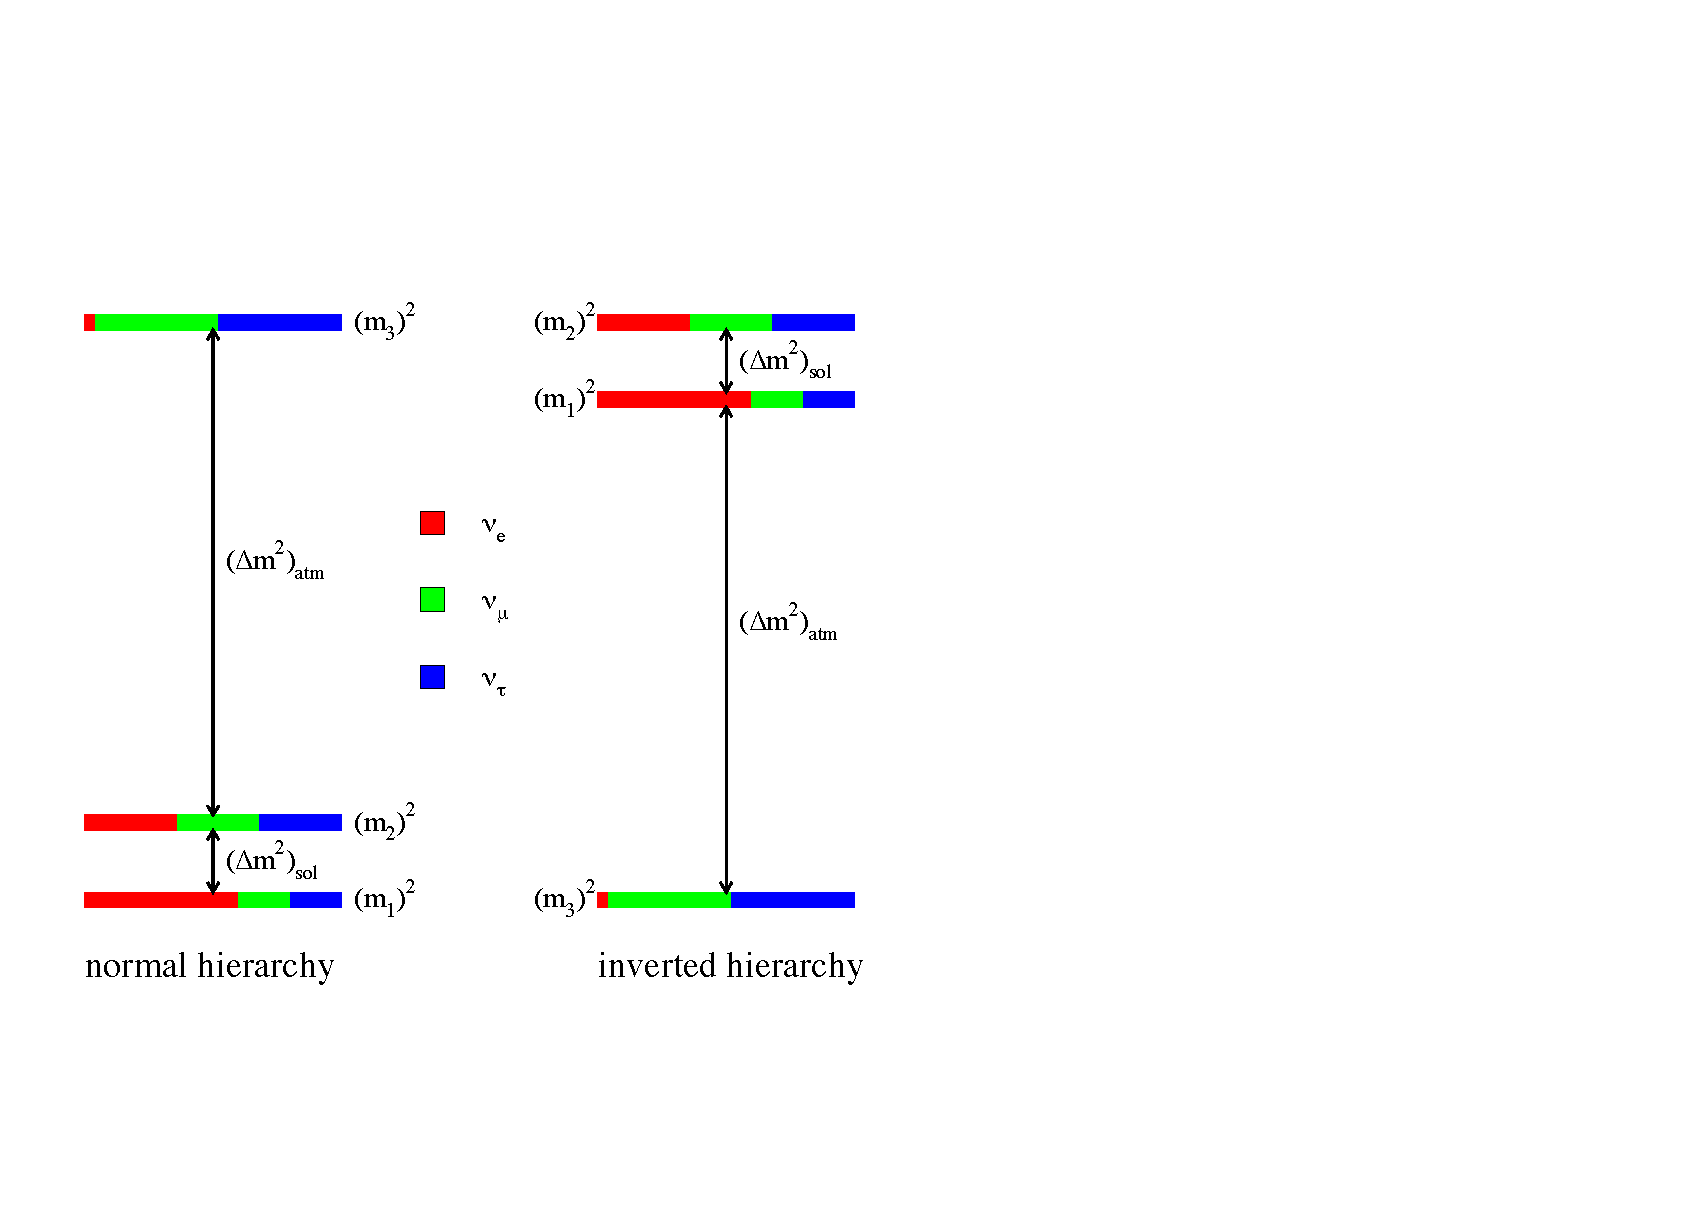
\includegraphics[width=0.8\textwidth]{./NuMass.pdf}
\end{figure}

How do we think we are going to measure the $\nu$\ mass hierarchy?

Two ways: \\

Most obvious way the hardest:  
There are actually 3 oscillation lengths.       
The mass differences are different. 
If we could see all three oscillation lengths, we would be able to determine the hierarchy.  
The Juno experiment in China is aimed at doing this. 
This is hard because you need a large distance to see the oscillation and very good resolution to see the short oscillation.
So you need a really big detector with very good resolution (These are usually competing requirements) 

The second way is through the matter effects. 
The basic idea is that \nue s behaves differently in matter (there are electrons around). 
This leads to an effect that depends on the sign of the $\Delta$m.
We didn't have time to cover this, look it up online.

\noindent\rule{\textwidth}{1pt}

\textbf{CP Violation:}  
There are two known sources of CP violations, one is in the quark sector where it is large another is in QCD where it is $\sim0$.
We don't understand this.  
If $\nu$s have mass there is another potential source of CP violation and we want to know if its big or small.

\noindent\rule{\textwidth}{1pt}

\textbf{$\nu$ masses}

Want to measure the $\nu$ masses

-Possible that the lightest is very nearly mass-less . \\
-Possible that all the masses are the same and the splittings are very small.

From a physics point of view this looks very different.
\bc
 Degenerate (split by a little bit)  vs  hierarchical 
\ec
The physics that might live behind that is different.

Measuring the masses has nothing to do with mixing: Cosmology / Particle physics 
 
beta decay spectra: KATRIN /  $10^{-12}$ / shape of the spectrum

\noindent\rule{\textwidth}{1pt}

\textbf{``Dirac vs Majorana``} 

How many $\nu$ DoFs ?  4 DoF  or 2 DoF? 

What prevents us from telling the difference ?

\textbf{If $m_e$ = 0}, we have two very different fields L and R completely unrelated to one another.
You would never connect them to one another. 
Only reason they are coupled is through the mass, there is an interaction that can transform a left-handed electron into a right-handed one.
That is how they are ``combined'' into a Dirac fermion.

\textbf{If $m_\nu$ = 0},
The left-handed nu and the ``would-be'' right-handed nu would be completely different particles. 
The right-handed nu in this scenario is a completely useless particle (no interactions at all)
The right-handed nu only manifested itself if $m_\nu$ != 0

They way you tell this is through neutrino-less double beta decay

 Z -> Z' + e + e 

 Z -> Z' + e + e  + nu + nu (very rare) has been observed (two neutrons decay at the same time) 


\noindent\rule{\textwidth}{1pt} 

\textbf{Why are people excited about $\nu$ physics? }

Have discovered that $\nu$ masses exist. 
Most amazing thing is that they are really small. 
Small compared to any masses you can think of. 

\begin{figure}[h!]
\centering
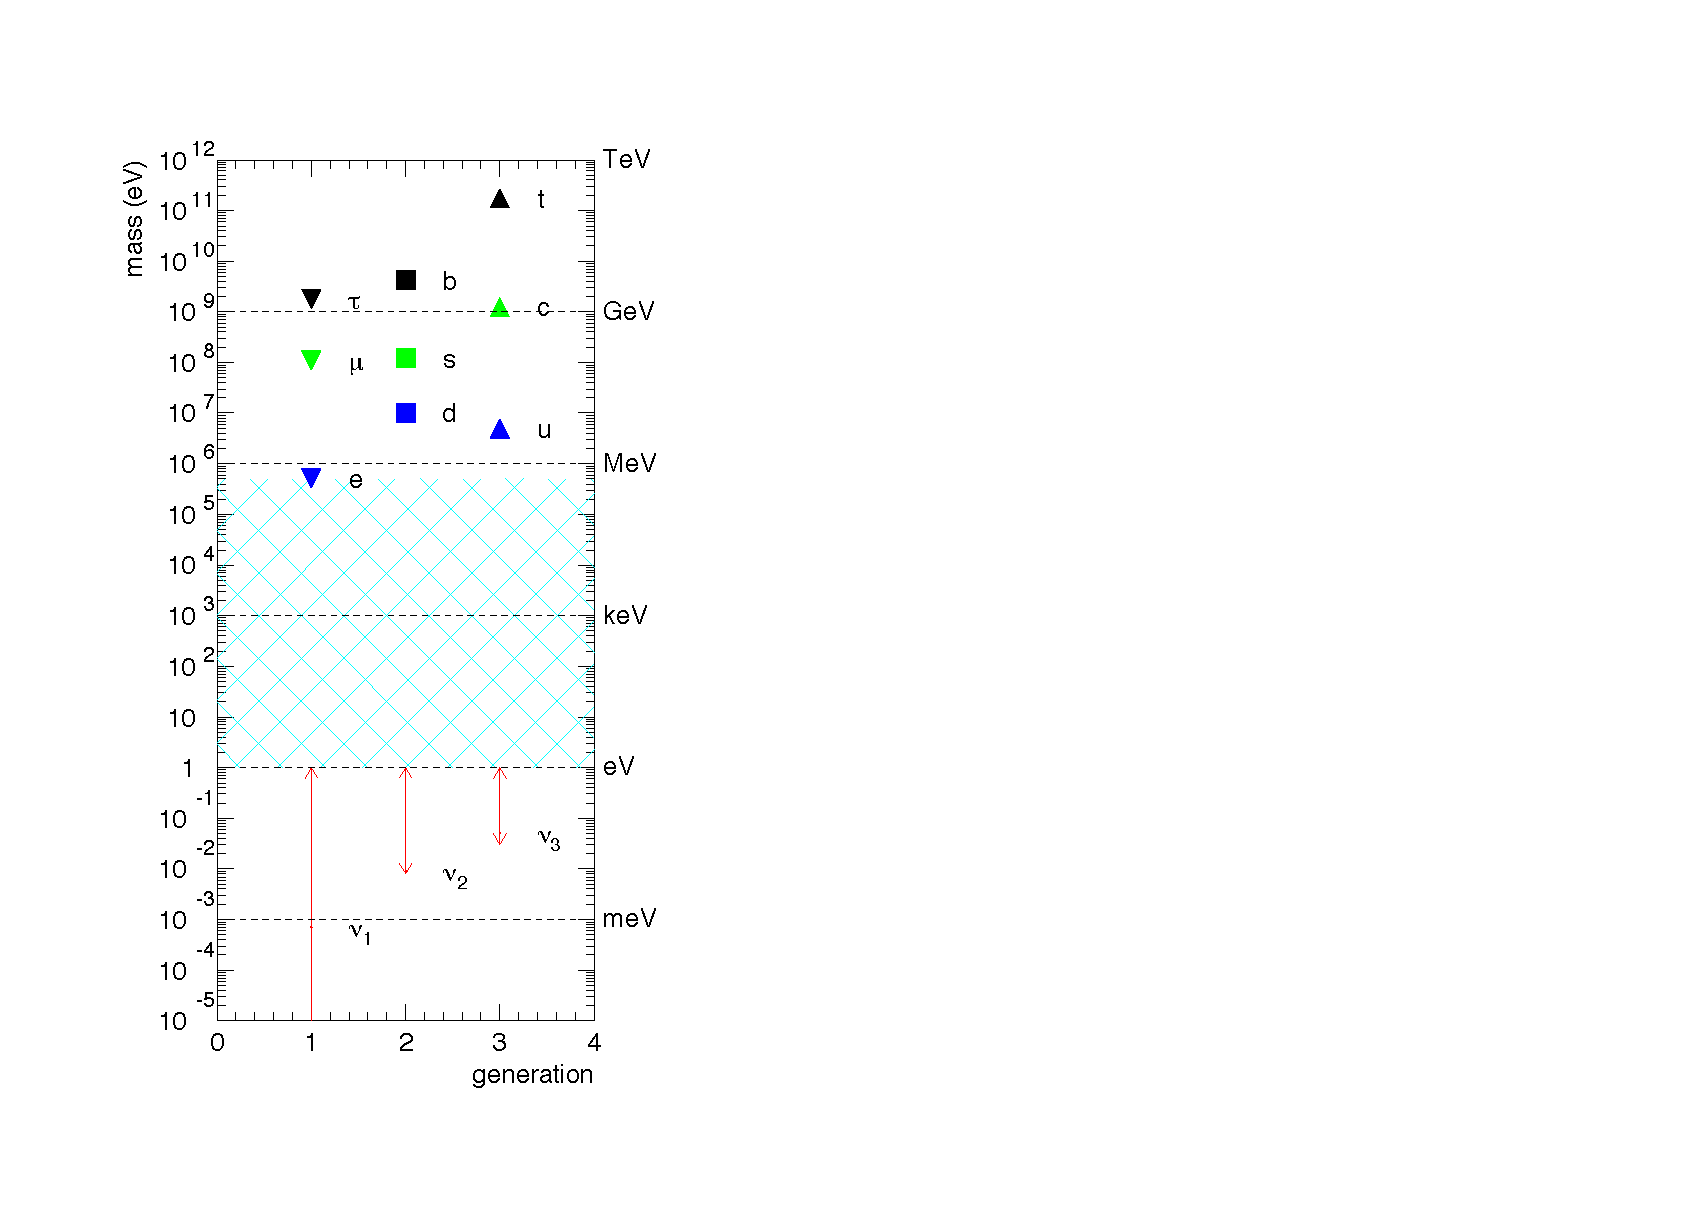
\includegraphics[width=0.5\textwidth]{./NuMass2.pdf}
\end{figure}


One of the biggest embarrassment in particle physics is the log plot below.
Masses are very different. 
All fundamental as far as we can tell. 
Masses span 16 orders of magnitude. 
$\nu$s are responsible for more than 1/2 that span. 

Spent a long time trying to understand why other fermion masses are so different. 
Haven't gotten anywhere. 
Now \nus\ live way down at the bottom.

Another strange thing, the charged fermion mass range is nicely populated. 
So every once in a while if your doing physics vs E you would run into a new fermion. 
Life is interesting. 
Particle physics in 60 and 70s. 

The gap between the heaviest $\nu$ and the electron is bigger than the difference between the electron and the top quark mass. 
What does any of this mean ? 
We have no idea.
Looks like something important.
So a lot of time is spent thinking about this.

Why are we excited about $\nu$ masses? 
\begin{itemize}
\item[-] Very small
\item[-] qualitatively different (?)
\end{itemize}

Everything is speculative...

%- Majorana fermions \\
%- In SM $m_\nu$ = 0.  (something we get very excited about) 

\noindent\rule{\textwidth}{1pt}

\textbf{Why did we believe $m_\nu$ = 0 in the SM ?}

Given the SM how do we give $\nu$s a mass ?

$m_\nu$> 0 mean new DoF.

Given, 
\bc
Q u d L e  + H + SU(3) x SU(2) x U(1)
\ec
you can write down an unambiguous Lagrangian.\\
This Lagrangian will give you $m_\nu$ = 0.

If you want to make $m_\nu$ > 0, something in this line has to change. 

One way, assume that the SM is an effective theory. 
Can keep playing the same game and write down higher dimensional operators. 

Start at dimension 5. 
Turns out there is only one dim-5 operator. 

(LH)(LH)/M + O(dim-6) 

What does this operator do ?
IF M is high enough, this operator does only one thing:
\bc
H gets a vev:   $L \sim  v^2 \nu^2 / M   = m_\nu  \nu^2$
\ec

This theory predicts that the first thing you should see is a non-zero $m_\nu$. 
\bc
$m_\nu = v^2 / M$
\ec
what makes this interesting is that this mass is parameterically different from charged fermion masses, 
\bc
 $m_l \propto v$   whereas $m_\nu \propto v^2$
\ec

This would ``explain'' why the $m_\nu$s are qualitatively different. 

So you could have written down this theory,  predict that $m_\nu$>0 is first sign of new physics, predict that $m_\nu$s are very small, and will predict that they are majorana masses. 

Very old idea (Wienberg '79) 

Most everyone is willing to bet that this is how $m_\nu$s happen. 
Sounds so plausible.

Required new DoF and some new Mass scale M.  
Could be very heavy.
$L \sim 10^{14}$ GeV 

This is one general idea. 

\noindent\rule{\textwidth}{1pt} 

Another general idea. 

More mundane, but will try convince you why this is interesting. 

%Well talk next week the plank scale, L sim $10^{14}$ GeV way below the $m_{plank}$. 

Other option is to mess around with the particle content in the SM.
Two options, add stuff to the fermion content or add stuff to the Higgs content. 
The higgs part is pretty easy, wont discuss that here.

%Add a triplet. 
%
%LTL majorana mass,  private higgs to the nus. 
%The triplet vev is very small so its probably OK. 
%
%All kinds of problems with the triplet. 
%T has lepton number, if lepton number symetry is not explictly broken it becomes can do this by adding new particles. 

Other way is the way everyone thinks of: Include right-handed nus:   $\nu^R$. 

These don't interact have no Quantum numbers. 
But you can right down a Yukawa interaction term:
\bc
$L \supset  y LHv $
\ec

after electro-weak symmetry breaking, 
$m_\nu  \sim y v$    ($y \sim10^{-12}$ not disallowed,  but weird. $y_e$ is $\sim10^{-6}$ and we've lived with that.)

Why is this model interesting? 
(Theory prejudice comes into play)

Could right down SM with: 
Q u d L e  + H + SU(3) x SU(2) x U(1)

Stopped at the dimension-4 level. 

If you add $\nu^R$ and play the same game, you get the Yukawa term but that's not the full Lagrangian.
You're missing a term. 

Can also write down a term like $L \supset \frac{M}{2} \nu^2$. 
This is allowed.
M would be a new mass scale in the SM, not connected to the Higgs. 

Qualitatively different from the L we had before. 
Question becomes, if you allow for $\nu_R$, should allow for the possibility that these mass terms exist. 
Depending on what those mass term are the phenomenology is very different. 

What happens in general don't know how many $\nu_R$s should exist. (Maybe 3, need at least 2) 
Lets say 3, then L predicts the existence of six neutral objects, masses Majorana fermions.

If $M >> yv$, then you can integrate out the have neutrino,

$L \sim y^2 LH^2 / M$  (Weinberg operator) 
Three light + three heavy. 

M > eV / all OK except cosmology 
  > MeV / cosmology OK

\noindent\rule{\textwidth}{1pt}

Another option is M = 0, allowed to do this. 
If the L has lepton number symmetry this number is exactly 0. 
 $\Rightarrow$ Lepton number is a fundamental symmetry of nature. 

Very different then how we look at lepton number today. 
In the SM, no where do I ask for Lepton Number (or Baryon Number) conservation. 
It just happens. 
This would be new. 


  

}
\end{document}


